% ==================================================================================================

\chapter{Implementation}
\label{ch:impl}

In the previous three chapters, we presented the theory of coeffects consisting of type system
and comonadically inspired semantics of two parameterized coeffect calculi. The theory provides
a framework that simplifies the implementation of safe context-aware programming languages. To
support this claim, this chapter presents a prototype implementation of three coeffect languages --
language with implicit parameters and both flat and structural versions of a data-flow language.

The implementation directly follows the thoery presented in the previous three chapters. It
consists of a common framework that provides type checking and translation to a simple functional
target language with comonadically-inspired primitives. Each concrete context-aware language then
adds a domain-specific rule for choosing unique typing derivation (as discussed in
Section~\ref{sec:flat-unique}) together with a domain-specific definition of the
comonadically-inspired primitives that define the runtime semantics (see Section~\ref{sec:semantics-proofs}).

The main goal of the implementation is to show that the theory is practically useful and to present it
in a more practical way. However, we do not intend to build a complete real-world programming language.
For this reason, the implementation is available primarilly as an interactive web-based essay, though
it can be also downloaded and run locally.

\paragraph{Chapter structure and contributions}

\begin{itemize}
\item We discuss how the implementation follows from the theory presented earlier (Section~\ref{sec:impl-theory}).
  This applies to the implementation of the \emph{type checker} and the implementation of the \emph{translation}
  to a simple target langauge that is then iterpereted. We also discuss how the common framework makes it
  easy to implement additional context-aware languages (Section~\ref{sec:impl-theory-ext}).

\item We consider a number of case studies (Section~\ref{sec:impl-case}) that illustrate interesting
  aspects of the theories discussed earlier. This includes the typing of lambda abstraction and the
  difference between flat and structural systems (Section~\ref{sec:impl-case-typing}) and the
  comonadically-inspired translation (Section~\ref{sec:impl-case-transl}).

\item The implementation is available not just as downloadable code, but also in the format of
  interactive web-based essay (Section~\ref{sec:impl-essay}), which aims to make coeffects
  accessible to a broader audience. We discuss the most interesting aspects of the essay format and
  briefly discuss some of the interesting implementation detail (Section~\ref{sec:impl-essay-tech}).
\end{itemize}


% ==================================================================================================
%
%    #######
%       #    #    # ######  ####  #####  #   #
%       #    #    # #      #    # #    #  # #
%       #    ###### #####  #    # #    #   #
%       #    #    # #      #    # #####    #
%       #    #    # #      #    # #   #    #
%       #    #    # ######  ####  #    #   #
%
% ==================================================================================================

\section{From theory to implementation}
\label{sec:impl-theory}

The theory discussed so far provides the two key components of the implementation. In
Chapter~\ref{ch:flat}, we discussed the type checking of context-aware programs and
Chapter~\ref{ch:semantics} models the execution of context-aware programs (in terms of
translation and operational semantics). For structural coeffects, the same components are discussed
in Chapter~\ref{ch:structural}. In this section, we discuss how those provide foundation for the
implementation.

% --------------------------------------------------------------------------------------------------

\subsection{Type checking and inference}
\label{sec:impl-theory-typing}

To simplify the writing of context-aware programs, the implementation provides a limited form of
type inference (Section~\ref{sec:impl-tech}). This is available just for convenience and so we do
not claim any completeness or complexity result about the algorithm and we do not present full
formalization. However, it is worth noting how the domain-specific procedures for choosing a unique
type derivation (Section~\ref{sec:flat-unique}) are adapted.

The type inference works in the standard way \cite{types-mlessence,types-inference} by generating
type constraints and solving them. Solving of type constraints is done in the standard way, but we
additionally collect and solve \emph{coeffect constraints}. In order to obtain unique type
derivation, we generate additional coeffect constraints in lambda abstraction of each flat
coeffect language.

\paragraph{Flat implicit parameters.}

As discussed in Section~\ref{sec:flat-unique}, when choosing unique typing derivation for
implicit parameters, we keep track of the implicit parameters available in lexical scope
(written as $\cclrd{\Delta}$). In lambda abstraction rule, the implicit parameters required by
the body (tracked by $\ccclrd{r}$) are split so that all parameters available in lexical scope
are captured and only the remaining parameters ($\cclrd{r}\setminus\cclrd{\Delta}$) are required
from the caller of the function.

From the presentation in Section~\ref{sec:flat-unique}, it might appear that resolving the ambiguity
related to lambda abstraction for implicit parameters requires a type system different from
the core flat coeffect type system shown earlier in Section ~\ref{sec:flat-calculus-types}.
This is not the case.

We track implicit parameters in scope $\cclrd{\Delta}$, but the rest of the (\emph{abs}) rule from
the implementation only generates an additional coeffect constraint. Writing
$\coctx{\Gamma}{\cclrd{t}} \vdash e : \tau ~|~ C}$ for a judgement that generates coeffect
constraints $C$, the (\emph{abs}) rule used for implicit parameters looks as follows:
%
\begin{equation*}
\tyrule{abs}
  {\coctx{\Gamma, x\!:\!\tau_1;\cclrd{\Delta}}{\cclrd{t}} \vdash e : \tau_2 ~|~ C}
  {\coctx{\Gamma;\cclrd{\Delta}}{\cclrd{r}} \vdash \lambda x\!:\!\tau_1.e : \tau_1 \xrightarrow{\cclrd{s}} \tau_2 ~|~
    C\cup\{\cclrd{t}=\cclrd{r} \,\czip\, \cclrd{s}, \cclrd{r}=\cclrd{\Delta} \}}
\end{equation*}
%
Given a typing derivation for the body that produced constraints $C$, we generate an additional
constraint that restricts $\cclrd{r}$ (declaration-site demands) to those available in the
current static scope $\cclrd{\Delta}$. It is not necessary to generate a constraint for the
coeffect $\cclrd{s}$, because our constraint satisfaction algorithm finds
the minimal set $\cclrd{s}$ which is $\cclrd{t}\cclrd{\setminus \Delta}$.

\paragraph{Flat data-flow.}
In context-aware language for data-flow (and in language with liveness tracking), the inherent
ambiguity of the (\emph{abs}) rule is resolved by duplicating the context requirements of the body.
In Section~\ref{sec:flat-unique}, this was defined by replacing the standard coeffect (\emph{abs})
rule with a rule (\emph{idabs}) that uses an annotation $\cclrd{r}$ for the body of the function,
declaration-site coeffect and call-site coeffect.

As with implicit parameters, the implementation does not require changing the core (\emph{abs})
typing rule of the flat coeffect system. Instead, the unique resulution is obtained by generating
additional coeffect constraints:
%
\begin{equation*}
\tyrule{abs}
  {\coctx{\Gamma, x\!:\!\tau_1}{\cclrd{t}} \vdash e : \tau_2 ~|~ C}
  {\coctx{\Gamma}{\cclrd{s}} \vdash \lambda x\!:\!\tau_1.e : \tau_1 \xrightarrow{\cclrd{t}} \tau_2 ~|~
    C\cup\{\cclrd{t}=\cclrd{r} \,\czip\, \cclrd{s}, \cclrd{r}=\cclrd{t}, \cclrd{s}=\cclrd{t} \}}
\end{equation*}
%
Here, the two additional constraints restrict both $\cclrd{r}$ and $\cclrd{s}$ to be equal to the
coeffect of the body $\cclrd{t}$ and so the only possible resolution is the one specified by
(\emph{idabs}).

% --------------------------------------------------------------------------------------------------

\subsection{Execution of context-aware programs}
\label{sec:impl-theory-transl}

Context-aware programs are executed by translating the source program into a simple functional
target language. For simplicity, programs in the simple target language are then interpreted, but
they could equally be compiled using standard techniques for compiling functional code. The
translation follows the rules defined in Section~\ref{sec:semantics-translation} (for flat coeffect
languages) and Section~X (for structural coeffect languages). The result of the translation is a
program that consists of the following:

\begin{itemize}
\item {\sc Functional constructs.} Those include binary operations, tuples, let binding,
  constants, variables, function abstraction and application. The interpreter keeps a map of
  assignments for variables in scope and recursively evaluates the expression.

\item {\sc Comonadic operations.} Those are the comonadic primitives provided by indexed comonads --
  \ident{cobind}, \ident{counit} together with \ident{merge} and \ident{split} for flat coeffects
  or \ident{merge} and \ident{choose} for structural coeffects. The translation that produces these
  is shared by all context-aware languages, but their definition in the interpreter is
  domain-specific.

\item {\sc Domain-specific operations.} Each context-aware language may additionally include
  operations that model domain-specific operations. For data-flow, this is \ident{prev} (accessing
  past values) and for implicit parameters, this is \ident{letimpl} and \ident{lookup} for implicit
  parameter binding and access, respectively.
\end{itemize}

\noindent
The fact that the prototype implementation is based on the theoretical framework provided by
coeffect calculi means that it has the desirable properties proved in Section~\ref{sec:semantics-proofs}
and Section~X. In particular, evaluating a well-typed context-aware program in a context that
provides sufficient contextual capabilities will not cause an error.

In the interactive essay (Section~\ref{sec:impl-essay}), we further use the coeffects to
automatically generate a user interface that requires the user to provide the required contextual
capabilities (past values for individual variables, or values for implicit parameters).

Another benefit of using the common framework is that the implementation can be easily extended
to support additional context-aware languages.

% --------------------------------------------------------------------------------------------------

\subsection{Supporting additional context-aware languages}
\label{sec:impl-theory-ext}

The prototype implementation supports two of the context-aware languages discussed in this thesis:
implicit parameters and data-flow. The remaining examples are calculus for tracking variable
liveness (of ordinary variables) and the structural language based on bounded reuse (counting
number of times values are used). However, the prototype implementation is based on the
common coeffect framework and makes it easy to add support for these and also for other context
aware languages based on coeffects.

In order to extend the implementation with support for liveness or bounded reuse tracking (or
other context-aware language), the following 4 additions are required:

\begin{enumerate}
\item A domain-specific function abstraction rule that resolves the ambiguity in the general
  (\emph{abs}) rule of the flat coeffect calculus. For liveness, the handling would be the same
  as for data-flow, but for other flat coeffect systems, another resolution mechanism might be used
  instead.

\item A domain-specific instance of coeffect algebra needs to be provided. In order to support
  the type inference in the prototype implementation, the constraint solver needs to be extended
  to solve constraint using the coeffect algebra. For liveness, this would be solving simple
  two-point lattice constraints.

\item For evaluation, a new kind of comonadic values needs to be added. For liveness, this would be
  an option value that may or may not contain a value. The semantics of comonadic operations on the
  values needs to be defined.

\item For context-aware languages that have additional primitives (such as \kvd{prev} or \ident{?param}),
  the parser and AST needs to be extended, custom type-checking and translation rules added and
  domain-specific primitive operations (with their semantics) provided. Liveness and bounded reuse
  do not have additional custom syntax and so supporting these would not require this step.
\end{enumerate}

\noindent
The list mirrors a list of steps that need to be done when supporting a new effectful computation
in a language that supports monadic do-notation. The step (3) corresponds to implementing a new
monad and (4) corresponds to adding monad-specific effectful operations. The step (2) applies when
using indexing to track effects more precisely \cite{effects-embedding}. The only step that does not
have effectful/monadic counterpart is (1).

When adding a new context-aware programming language support, much of the existing infrastructure
can be reused. This includes the implementation of the core coeffect and type checking rules and
also the translation for standard language constructs as well as the interpreter for the target
language.


% ==================================================================================================
%
%     #####
%    #     #   ##    ####  ######     ####  ##### #    # #####  # ######  ####
%    #        #  #  #      #         #        #   #    # #    # # #      #
%    #       #    #  ####  #####      ####    #   #    # #    # # #####   ####
%    #       ######      # #              #   #   #    # #    # # #           #
%    #     # #    # #    # #         #    #   #   #    # #    # # #      #    #
%     #####  #    #  ####  ######     ####    #    ####  #####  # ######  ####
%
% ==================================================================================================

\section{Case studies}
\label{sec:impl-case}

The prototype implementation illustrates a number of interesting aspects of coeffect systems.
Those appear as examples in the interactive essay (discussed in Section~\ref{sec:impl-essay}), but
we briefly review them in this section.

% --------------------------------------------------------------------------------------------------

\subsection{Typing context-aware programs}
\label{sec:impl-case-typing}

We first consider two case studies of how coeffect type checking works. The first one exposes the
resolution of the ambiguity in typing for implicit parameters and the second one exposes the
difference between flat and structural system for data-flow.

\paragraph{Abstraction for implicit parameters.}
As discussed in Section~\ref{sec:impl-theory-typing}, the implementation of the language with
implicit parameters resolves the ambiguity in the lambda abstraction by generating a coeffect
constraint that restricts the set of parameters required from the declaration-site to those that
are lexically available. Remaining parameters are required from the call-site. This is illustrated
by the following example:
%
\begin{equation*}
\begin{array}{l}
\kvd{let}~\ident{both}~=\\[-0.25em]
\quad \kvd{let}~\ident{?fst}~=~100~\kvd{in}\\[-0.25em]
\quad \kvd{fun}~\ident{trd}~\rightarrow~\ident{?fst}~+~\ident{?snd}~+~\ident{trd}~\kvd{in}\\[-0.25em]
\kvd{let}~\ident{?fst}~=~200~\kvd{in}\\[-0.25em]
\ident{both}~1
\end{array}
\end{equation*}
%
In this expression, the lambda function on line 3 requires implicit parameters \ident{?fst} and
\ident{?snd}. Since \ident{?fst} is available in scope, the type of \ident{both} is a function that
requires only \ident{?snd}. In the text-based notation used in the prototype, the type of the
function \ident{both} is: {\tt num -\{?snd:num\}-> num}.

\paragraph{Flat and structural data-flow.}
In flat data-flow, the context requirements of the body is required from both the declaration-site
and from the call-site. In structural data-flow, the context requirements are tracked separately
for each variable, which provides a more precise type. Consider the following two examples (the
\kvd{let} keyword is used to define a curried function of two arguments):
%
\begin{equation*}
\begin{array}{l}
\kvd{let}~\ident{oldy}~\ident{x}~\ident{y}~=~\ident{x}~+~\kvd{prev}~\ident{y}~\kvd{in}\\[-0.25em]
\ident{oldy}
\end{array}
\end{equation*}
%
When type checking the expression using the flat system, the type of \ident{oldy} is inferred as {\tt num -\{1\}-> num -\{1\}-> num},
but when using the structural system, the type becomes {\tt num -\{0\}-> num -\{1\}-> num}.

This illustrates the difference between the two - the flat system keeps only one annotation
for the whole body (which requires 1 past value). In lambda abstraction (or function declaration
written using \kvd{let}), this requirement is duplicated. The structural system keeps information
per-variable and so the resulting type reflects the fact that only the variable \idnet{y} appears
inside \kvd{prev}.

% --------------------------------------------------------------------------------------------------

\subsection{Comonadically-inspired translation}
\label{sec:impl-case-transl}

In addition to running coeffect programs, the implementation can also print the result of the
translation to the simple functional target language with comonadically-inspired primitives.
The following two case studies illustrate important aspects of the translation for flat coeffect
systems (Section~\ref{sec:semantics-translation}) and structural coeffect systems (Section~?).

\paragraph{Merging implicit parameter contexts.}

The following example illustrates the lambda abstraction for implicit parameters.
It defines a parameter \ident{?param} and then returns a function value that captures it, but
also requires an implicit parameter \ident{?other}:
%
\begin{equation*}
\begin{array}{l}
\kvd{let}~\ident{?param} ~=~ \num{10}~\kvd{in}\\[-0.25em]
\kvd{fun}~\ident{x}~\rightarrow~\ident{?param} ~+~ \ident{?other}
\end{array}
\end{equation*}
%
Translating the code to the target language produces the code below. The reader is encouraged to
view the translation in the interactive essay (Section~\ref{sec:impl-essay}), which displays the
types and coeffect annotations of the individual values and primitives. As in the theory, the
comonadically-inspired primitives are families of operations indexed by the coeffects (we
omit the annotations here):
%
\begin{equation*}
\begin{array}{l}
\kvd{let}~(\ident{ctx2}, \ident{ctx3}) ~=~ \ident{split}~(\ident{duplicate}~\kvd{finput})~\kvd{in}\\[-0.25em]
\kvd{let}~\ident{ctx1} ~=~ \ident{letimpl}_{\ident{?param}}~(\ident{ctx2}, \num{10})~\kvd{in}\\[-0.25em]
\kvd{fun}~\ident{x}~\rightarrow\\[-0.25em]
\quad \kvd{let}~\ident{ctx4} ~=~ \ident{merge}~(\ident{x}, \ident{ctx1})~\kvd{in}\\[-0.25em]
\quad \kvd{let}~(\ident{ctx5}, \ident{ctx6}) ~=~ \ident{split}~(\ident{duplicate}~\ident{ctx4})~\kvd{in}\\[-0.25em]
\quad \ident{lookup}_{\ident{?param}}~\ident{ctx5} ~+~ \ident{lookup}_{\ident{?other}}~\ident{ctx6}
\end{array}
\end{equation*}
%
The \kvd{finput} value on the first line represents an empty context in which the expression is
evaluated and is of type $\ctyp{\czero}{\ident{unit}}$. The context is duplicated; \ident{ctx3}
is not needed, because $\num{10}$ is a constant; \ident{ctx2} is passed to \ident{letimpl}, which
assigns an implicit parameter value in the newly returned context \ident{ctx1} of type
$\ctyp{\cclrd{\{\ident{?param}\}}}{\ident{unit}}$ (this now carries the implicit parameter value, but
it does not represent any ordinary variables, thus the \ident{unit} type representing an empty
tuple).

In the body of the function, the context \ident{ctx1} is merged with the context provided by the
variable \ident{x}. The type of \ident{ctx4} is $\ctyp{\ccrld{\{\ident{?param},\ident{?other}\}}}{(\ident{num}\times\ident{unit})}$.
This is then split into two parts that contain just one of the implicit parameters and those are
then accessed using \ident{lookup}.

\paragraph{Composition in structural data-flow.}

In structural coeffect systems, the translation works differently in that the context passed to
a sub-expression contains only assignments for the variables used in the sub-expression (in the
flat version, we always duplicated the variable context before using \ident{split}). To illustrate
this, consider the following simple function:
%
\begin{equation*}
\begin{array}{l}
\kvd{fun}~\ident{x} \rightarrow \kvd{fun}~\ident{y} \rightarrow \kvd{prev}~\ident{x}
\end{array}
\end{equation*}
%
In structural coeffect systems, the comonadic value is annotated with a vector of coeffect
annotations that correspond to individual variables. The initial structural input \kvd{sinput}
is a value of type $\ctyp{\cclrd{[]}}{()}$ containing no variables (we write $()$ rather than
\ident{unit} to make that more explicit). The translated code then looks as follows:
%
\begin{equation*}
\begin{array}{l}
\kvd{fun}~\ident{x} \rightarrow\\[-0.25em]
\quad \kvd{let}~\ident{ctx1} ~=~ \ident{merge}~(\ident{x}, \kvd{sinput}) \kvd{in}\\[-0.25em]
\quad (\kvd{fun}~\ident{y} \rightarrow\\[-0.25em]
\quad \quad \kvd{let}~\ident{ctx2} ~=~ \ident{merge}~(\ident{y}, \ident{ctx1})~\kvd{in}\\[-0.25em]
\quad \quad \ident{counit}~(\ident{prev}~(\ident{choose}_{\langle 0,1\rangle}~\ident{ctx2}))
\end{array}
\end{equation*}
%
The two variables are merged with the initial context, obtaining a value \ident{ctx2} of type
$\ctyp{\cclrd{[0, 1]}}{\ident{num}\times\ident{num}}$ that contains two values with 0 and 1 past
values, respectively.

For simplicity, the implementation does not use the \ident{split}/\ident{merge} pair of operations
of the structural coeffects to obtain the correct subset of variables. This can be done, but it
would make the translated code longer and more cumbersome. Instead, we use a higher-level operation
\ident{choose} (which can be expressed in terms of \ident{split}/\ident{merge}) that projects the
variable subset as specified by the index. Here, $\langle 0, 1\rangle$ means that the first variable
should be dropped an the second one should be kept.

The resulting single-variable context is then passed to \ident{prev} (to shift the stream by one)
and then to \ident{counit} to obtain the current value.


% ==================================================================================================
%
%    #######
%    #        ####   ####    ##   #   #
%    #       #      #       #  #   # #
%    #####    ####   ####  #    #   #
%    #            #      # ######   #
%    #       #    # #    # #    #   #
%    #######  ####   ####  #    #   #
%
% ==================================================================================================

\section{Interactive essay}
\label{sec:impl-essay}

As explained in the introduction of this chapter, the purpose of the implementation presented in
this thesis is not to provide a real-world programming language, but to support the theory
discussed in the rest of the thesis. The goal is to explain the theory and inspire authors of
real-world programming langauges to include support for context-aware programming, ideally using
coeffects as a sound foundation. For this reason, the implementation needs to be:

\begin{itemize}
\item {\sc Accessible.}  Anyone interested should be able to use the implemented langauges without
  downloading the source code and compiling it and without installing specialized software.

\item {\sc Explorable.}  It should be possible to explore the inner workings -- how is the typing
  derived, how is the source code translated to the target language and how is it evaluated.
\end{itemize}

\noindent
To make the work \emph{accessible}, we implement sample context-aware languages in a way that makes it
possible to use them in any standard web browser with JavaScript support (Section~\ref{sec:impl-essay-tech})
without requiring any server-side component. Following the idea that ``the medium is the message'' \cite{essay-medium},
we choose medium that encourages \emph{exploration} and make the implementation available not just
as source code that can be compiled and run locally, but also in the format of
interactive essay (Section~\ref{sec:impl-essay-features}). The live version of the essay can be
found at: \url{http://tomasp.net/coeffects}.

% --------------------------------------------------------------------------------------------------

\begin{figure}[t]
\boxed{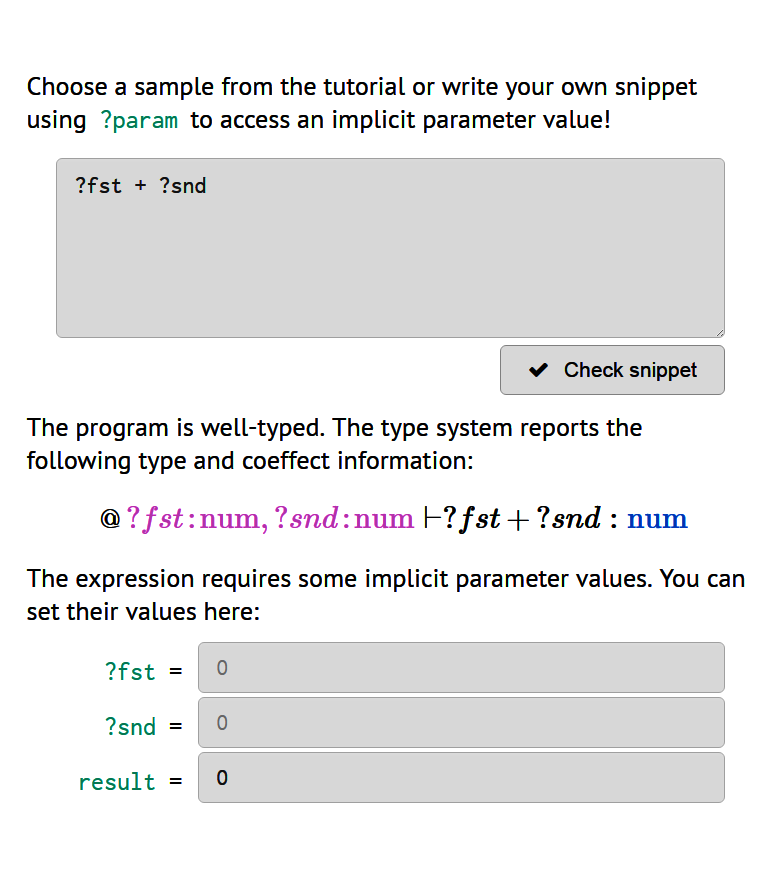
\includegraphics[width=16em]{images/eval1.png}}
\boxed{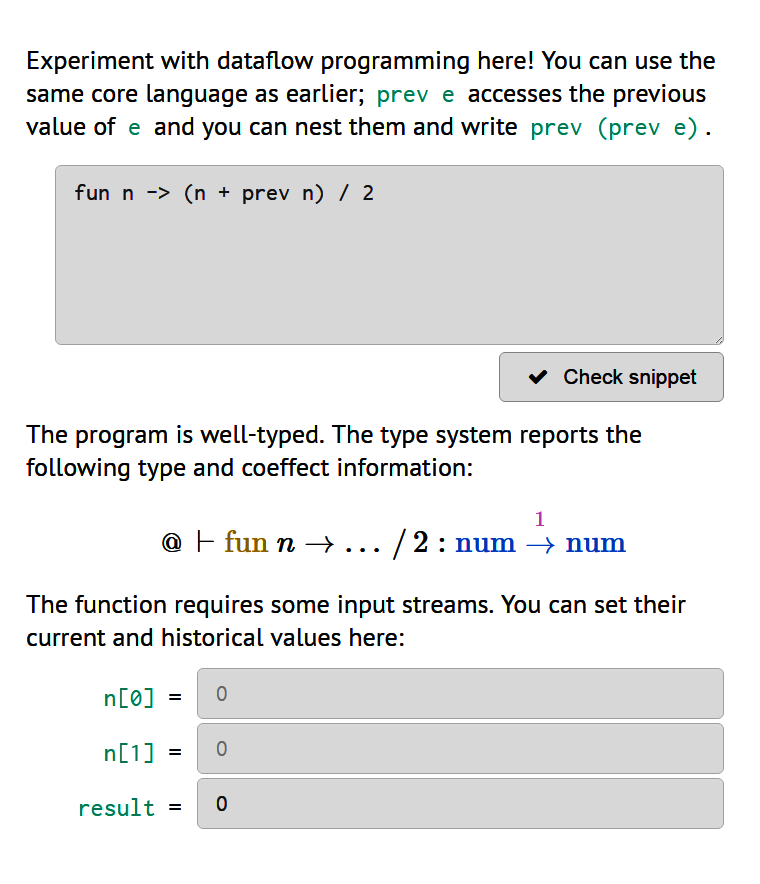
\includegraphics[width=16em]{images/eval2.png}}
\caption{Interactive evaluation of implicit parameters (left) and data-flow (right)}
\label{fig:essay-eval}
\end{figure}

% --------------------------------------------------------------------------------------------------

\subsection{Explorable language implementation}
\label{sec:impl-essay-features}

The interactive essay format used of the implementation is inspired by Bret Victor's work on
\emph{explorable explanations} \cite{essay-explorable}:
%
\begin{quote}
\emph{Do our reading environments encourage active reading? Or do they utterly oppose it? A
  typical reading tool, such as a book or website, displays the author's argument, and nothing
  else. The reader's line of thought remains internal and invisible, vague and speculative. We
  form questions, but can't answer them. We consider alternatives, but can't explore them. We
  question assumptions, but can't verify them. And so, in the end, we blindly trust, or blindly
  don't, and we miss the deep understanding that comes from dialogue and exploration.}
\end{quote}
%
The interactive essay we present encourages active reading in the sense summarized in Victor's quote.
We show the reader an example (program, typing derivation or translation), but the reader is
encouraged to modify it and see how the explanation in the essay adapts.

The idea of active reading is older and has been encouraged in the context of art Josef Albers'
classic 1963 work on color \cite{essay-albers} (which has been turned into an interactive essay
60 years later \cite{essay-albers-app}). More recently, similar formats have been used to explain
topics in areas such as signal processing \cite{essay-seeing} (explaining Fourrier transformations)
and sociology \cite{essay-polygons} (visualizing and explaining game theoretical model of segregation
in the society \cite{essay-segregation}). To our best knowledge, no such work exists in the area
of programming language theory and so we briefly outline some of the interesting features that
our essay provides in order to encourage active reading.

\paragraph{Interactive program excution.}

After providing the practical motivation for coeffects (based on Chapter~\ref{ch:intro}), the
interactive essay shows the reader the two sample context-aware programming languages. Readers can
write code in a panel that type checks the input, generates user interface for entering the
required context and runs the sample code.

The panels for implicit parameters and for data-flow computations are shown in Figure~\ref{fig:essay-eval}.
The sample code on the left adds two implicit parameters and the generated UI lets the user
enter implicit parameter values as required by the context in the typing judgement. The sample on
the right calculates the average of the current and past value in a data-flow; the UI lets the user
enter past values required by the type of the function.

The essay guides the readers through a number of interesting programs (shown in Section~\ref{sec:impl-case-typing})
and encourages them to run and try modifying them. For implicit parameters, this includes the case
where an implicit parameter is available at both declaration-site and call-site (showing that the
declaration-site value is captured). For data-flow, the examples include the comparison between the
inferred type when using flat and structural type systems.

% --------------------------------------------------------------------------------------------------

\begin{figure}[t]
\boxed{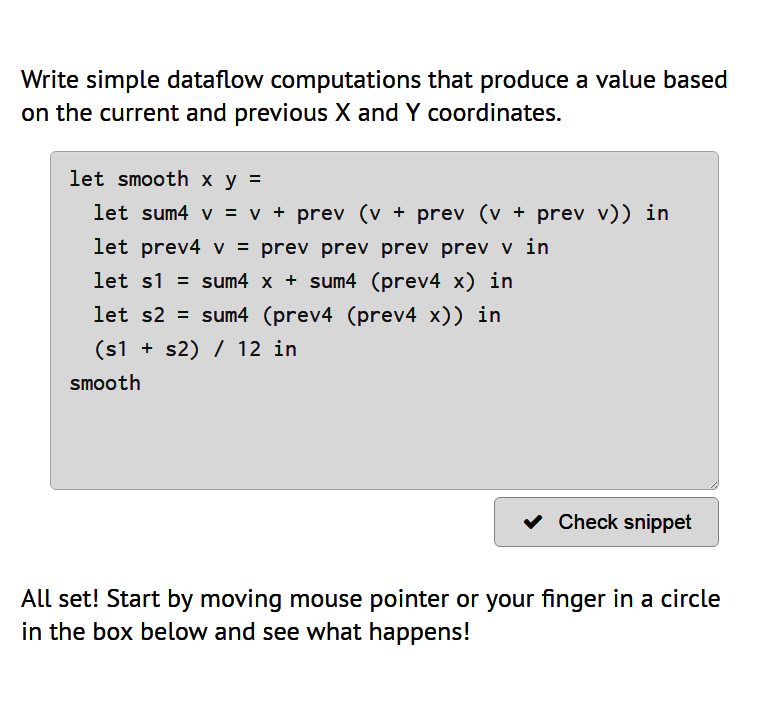
\includegraphics[width=16em]{images/df1.png}}
\boxed{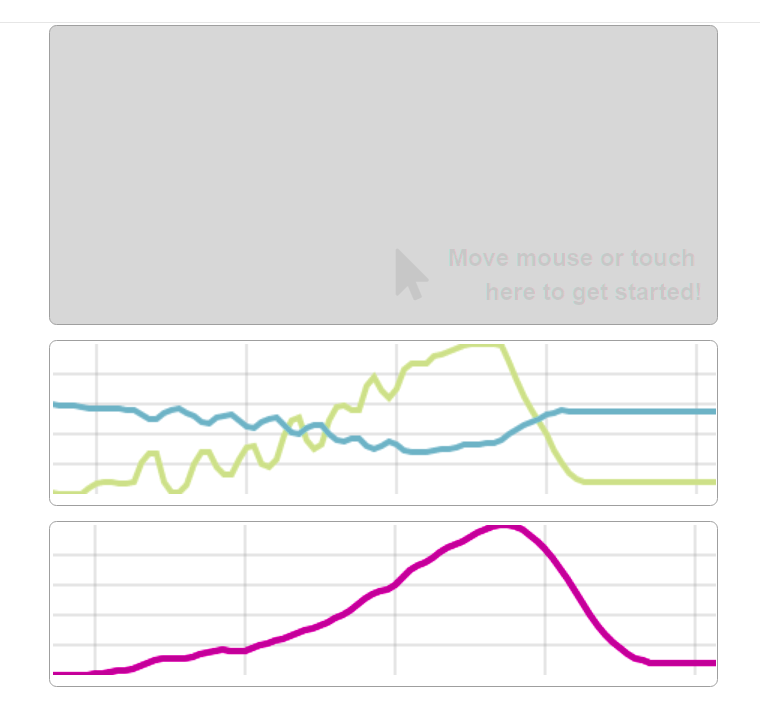
\includegraphics[width=16em]{images/df2.png}}
\caption{Function smoothing the X coordinate (left) with a sample run (right).}
\label{fig:essay-df}
\end{figure}

% --------------------------------------------------------------------------------------------------

\paragraph{Reactive data-flow.}

The interactive program execution lets the reader run sample programs, but not in a realistic
context. To show a more real-world scenario, the essay includes a widget shown in Figure~\ref{fig:essay-df}.
This lets the user write a function taking a stream of X and Y coordinates and calculate value
based on the current and past values of the mouse pointer. The X and Y values, together with the
result are plotted using a live chart.

In the example run shown above, the sample program calculates the average of the last 12 values
of the X coordinate (green line in Figure~\ref{fig:essay-df}). The example also illustrates one
practical use of the coeffect type system -- when running, the widget keeps the coordinates in a
pre-allocated fixed-size array, because the coeffect type system guarantees that at most 12 past
values will be accessed.

% --------------------------------------------------------------------------------------------------

\begin{figure}[t]
\boxed{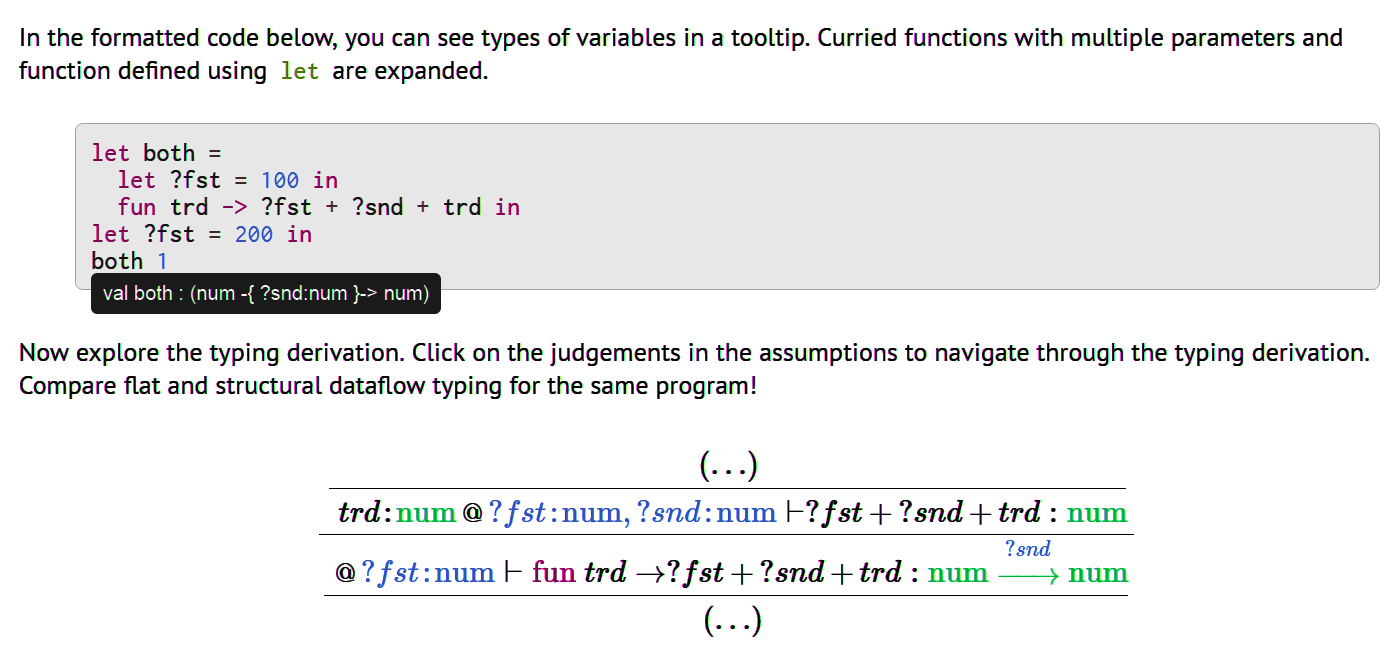
\includegraphics[width=32em]{images/types.png}}
\caption{Source code with type information and explorable typing derivation.}
\label{fig:essay-typing}
\end{figure}

% --------------------------------------------------------------------------------------------------

\paragraph{Explorable typing derivations.}

Perhaps the most important aspect of the implemented context aware programming languages is their
coeffect and type system. In a conventional implementation, the functioning of the type system
would remain mostly hidden -- we would get an ``OK'' message for a well-typed program and a type
error for invalid program (likely not very informative, given that reporting good error messages
for type errors is a notoriously hard problem even for mature language implementations).

The presented interactive essay provides two features to help the reader understand and explore
typing derivations. First, when reading code samples in the text, tooltips show the typing of
individual identifiers, most interestingly functions (Figure~\ref{fig:essay-typing}, above).

Second, a later part of the essay provides a type checker that lets the user enter a source code
in a context aware programming language and produces an explorable typing derivation for the
program. The output (shown in Figure~\ref{fig:essay-typing}, below) displays a typing judgement
with assumptions and conclusions and lets the reader navigate through the typing derivation by
clicking on the assumptions or conclusions. This way, the reader can see how is the final typing
derivation obtained, exploring interesting aspects, such as the abstraction rule (shown in
Figure~\ref{fig:essay-typing}).

\paragraph{Comonadically-inspired translation.}

The last interactive element of the essay lets the reader explore the translation of source
context aware language to a target simple functional language (Section~\ref{sec:impl-theory-transl}).
Compared with the monadic do-notation \cite{other-haskell98}, the comonadic translation is more
complex for two reasons. First, it merges all variables into a single (comonadic) value representing
the context. Second, there is a flat and structural variation of the system. For these two reasons,
understanding the translation based just on the rules is harder than for monads. The essay lets
readers see translation for carefuly chosen case studies that illustrate the key aspects of the
translation (some discussed in Section~\ref{sec:impl-case-transl}), but also for their own
programs encouraging \emph{active reading}. Sample input and output are shown in
Figure~\ref{fig:essay-transl}.


% --------------------------------------------------------------------------------------------------

\begin{figure}[t]
\boxed{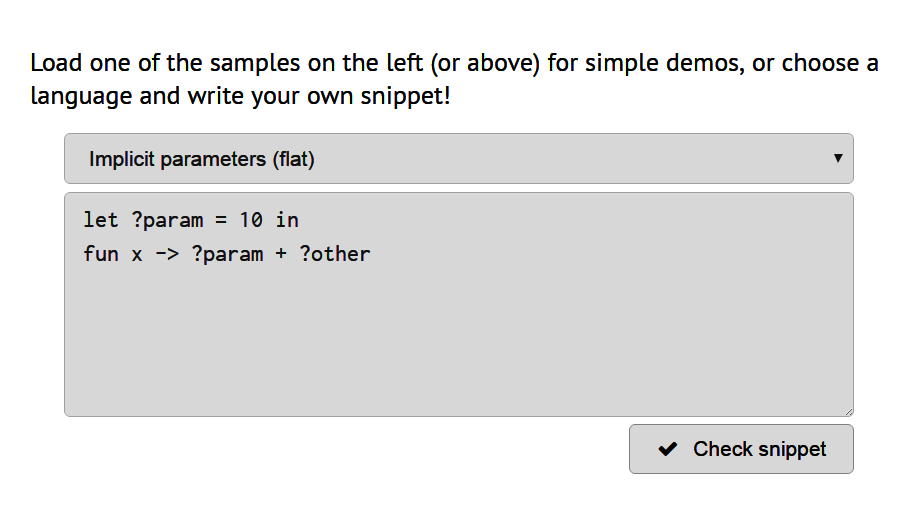
\includegraphics[width=16em]{images/transl1.png}}
\boxed{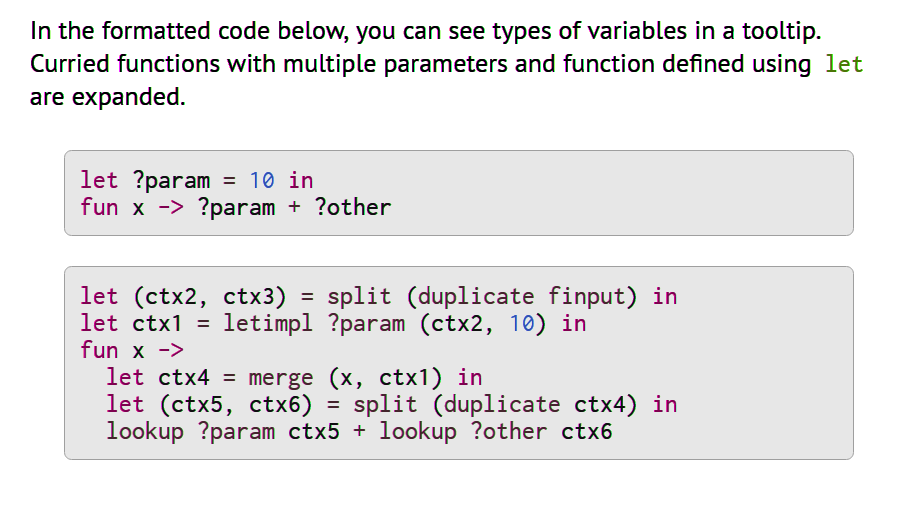
\includegraphics[width=16em]{images/transl2.png}}
\caption{TBD}
\label{fig:essay-transl}
\end{figure}

% --------------------------------------------------------------------------------------------------

\subsection{Implementation overview}
\label{sec:impl-essay-tech}

The core part of our implementation mostly follows standard techniques for implementing type
checkers and interpreters for statically-typed functional programming langauges. Two interesting
aspects that are worth discussing is the JavaScript targetting (for running the langauge
implementation in a web browser) and integration with client-side (JavaScript) libraries for
building the user interface. The full source code can be obtained from
\url{https://github.com/coeffects/coeffects-playground} and is structured as follows:
%
\begin{itemize}
\item Parsing is implemented using smple parser combinator library; \strf{ast.fs} defines the
  abstract syntax tree for the languages; \strf{parsec.fs} implements a small parser combinator
  library and \strf{lexer.fs} with \strf{parser.fs} parse the source code by first tokenizing
  the input and then parsing the stream of tokens.

\item The type checking is implemented by \strf{typechecker.fs}, which annotates an untyped AST
  with types and generates set of type and coeffect constraints. The constraints are later solved
  (using domain-specific algorithms for each of the languages) in \strf{solver.fs}.

\item Type-checked programs in context-aware languages are translated to simple target
  functional subset of the language in \strf{translation.fs}; \strf{evaluation.fs} then interprets
  programs in the target language. The interpretation does not handle the source
  language and so programs containing context-aware contstructs cannot be interpreted directly.

\item The user interface of the interactive essay discussed in Section~\ref{sec:impl-essay-features}
  is implemented partly in F\# and partly in JavaScript. The two most important components include
  a pretty-printer \strf{pretty.fs} which formats source code (with type tooltips) and typing
  derivations and \strf{gui.fs} that implements user interaction (e.g.~navigation in explorable
  typing derivations).
\end{itemize}

\noindent
As discussed in Section~\ref{sec:impl-theory-ext}, the implementation can be easily extended to
support additional context-aware programming languages. This is due to the fact that it is based
on the unified theory of coeffects. In practice, adding support for liveness tracking would
require adding a domain-specific constraint solver in \strf{solver.fs} and extending the
interpreter in \strf{evaluation.fs} with a new kind of comonadically-inspired data type
(indexed maybe comonad) with its associated operations.

\section{Related work}
\label{sec:impl-related}

To our best knowledge, combining Bret Victor's idea of explorable explanations with programming
language theory (as discussed in Section~\ref{sec:impl-essay}) is a novel contribution of our work.
On the technical side, we build on a number of standard methods.

\paragraph{Parsing and type checking.} The implementation of the parser, type checker and
interpreter follows standard techniques for implementing functional programming languages.
In order to be able to compile the implementation to JavaScript (see below), we built a
small parser combinator library \cite{monad-parsing} rather than using one of the already
available libraries \cite{other-fparsec}.

\paragraph{Targetting JavaScript.} In order to make the implementation accessible to a broad
audience, it can be executed in a web browser. This is achieved by automatically translating the
implementation from F\# to JavaScript. We use an F\# library called FunScript \cite{other-funscript}
(which is a more recent incarnation of the idea developed by the author \cite{app-fsharp-webtools}).
We choose F\#, but similar tools exist for other functional languages such as OCaml \cite{other-js-ocaml}.
It is worth noting that FunScript is implemented as a \emph{library} rather than as a compiler
extension. This is done using the meta-programming capabilities of F\# \cite{app-fsharp-metaprog}.

\paragraph{Client-side library integration.} An interesting aspect of the interactive essay
user interface is the integration with third-party JavaScript libraries. We use a number of
libraries including JQuery (for web browser DOM manipulation) and MathJax \cite{essay-mathjax}
(for rendering of typing derivation). In order to call those from F\# code, we use a number
of mapping methods described in \cite{app-age-of-web}. For example, the following F\# declaration
is used to invoke the \ident{Queue} function in MathJax:
%
\begin{equation*}
\begin{array}{l}
\lbrack\langle\ident{JSEmitInline}(\str{MathJax.Hub.Queue(\{0\});})\rangle\rbrack\\[-0.25em]
\kvd{let}~\ident{queueAction}~(\ident{f}:\ident{unit}~\rightarrow~\ident{unit}):\ident{unit}~=~\ident{failwith}~\str{JS only!}
\end{array}
\end{equation*}
%
The \ident{JSEmitInline} syntax on the first line is an attribute that instructs FunScript
to compile all invocations of the \ident{queueAction} function into the JavaScript literal
specified in the attribute (with \strf{\{0\}} replaced by the argument).


% ==================================================================================================
%
%     #####
%    #     # #    # #    # #    #   ##   #####  #   #
%    #       #    # ##  ## ##  ##  #  #  #    #  # #
%     #####  #    # # ## # # ## # #    # #    #   #
%          # #    # #    # #    # ###### #####    #
%    #     # #    # #    # #    # #    # #   #    #
%     #####   ####  #    # #    # #    # #    #   #
%
% ==================================================================================================

\section{Summary}

This chapter supplements the theory of coeffects presented in the previous three chapters with
a prototype implementation. We implemented three simple context-aware programming langauges that
track implicit parameters and past values in dataflow computations (in flat and structural way).

The implementation discussed in this chapter provides an evidence for our claim that the
theory of coeffects can be used as a basis for a wide range of sound context-aware programming
languages. Our implementation consists of a shared coeffect framework (handling type checking and
translation). Each context-aware language then adds a domain-specific rule for choosing a unique
typing derivation, an interpretation of comonadically-inspired primitives and (optionally)
domain-specific primitives such as the \kvd{prev} construct for dataflow.

We make the implementation available in the usual form (as source code that can be downloaded,
compiled and executed), but we also present it in the form of interactive essay. This encourages
\emph{active reading} and lets the reader explore a number of aspects of the implementation
including the type checking (through explorable typing derivations) and the translation. The key
contribution of this thesis is that it provides a unified way for \emph{thinking} about context in
programming langauges and the interactive presentation of the implementation is aligned with this
goal. Programming languages of the future will need a mechanism akin to coeffects and we aim to
provide a convincing argument supported by a prototype implementation.
